\documentclass{standalone}
\usepackage{tikz}
\usetikzlibrary{patterns}
\usetikzlibrary{positioning}
\usetikzlibrary{patterns, positioning}
\usetikzlibrary{shapes.misc}
\usepackage[outline]{contour}
\contourlength{1.5pt} 
\usepackage[sfdefault]{ClearSans}

\begin{document}
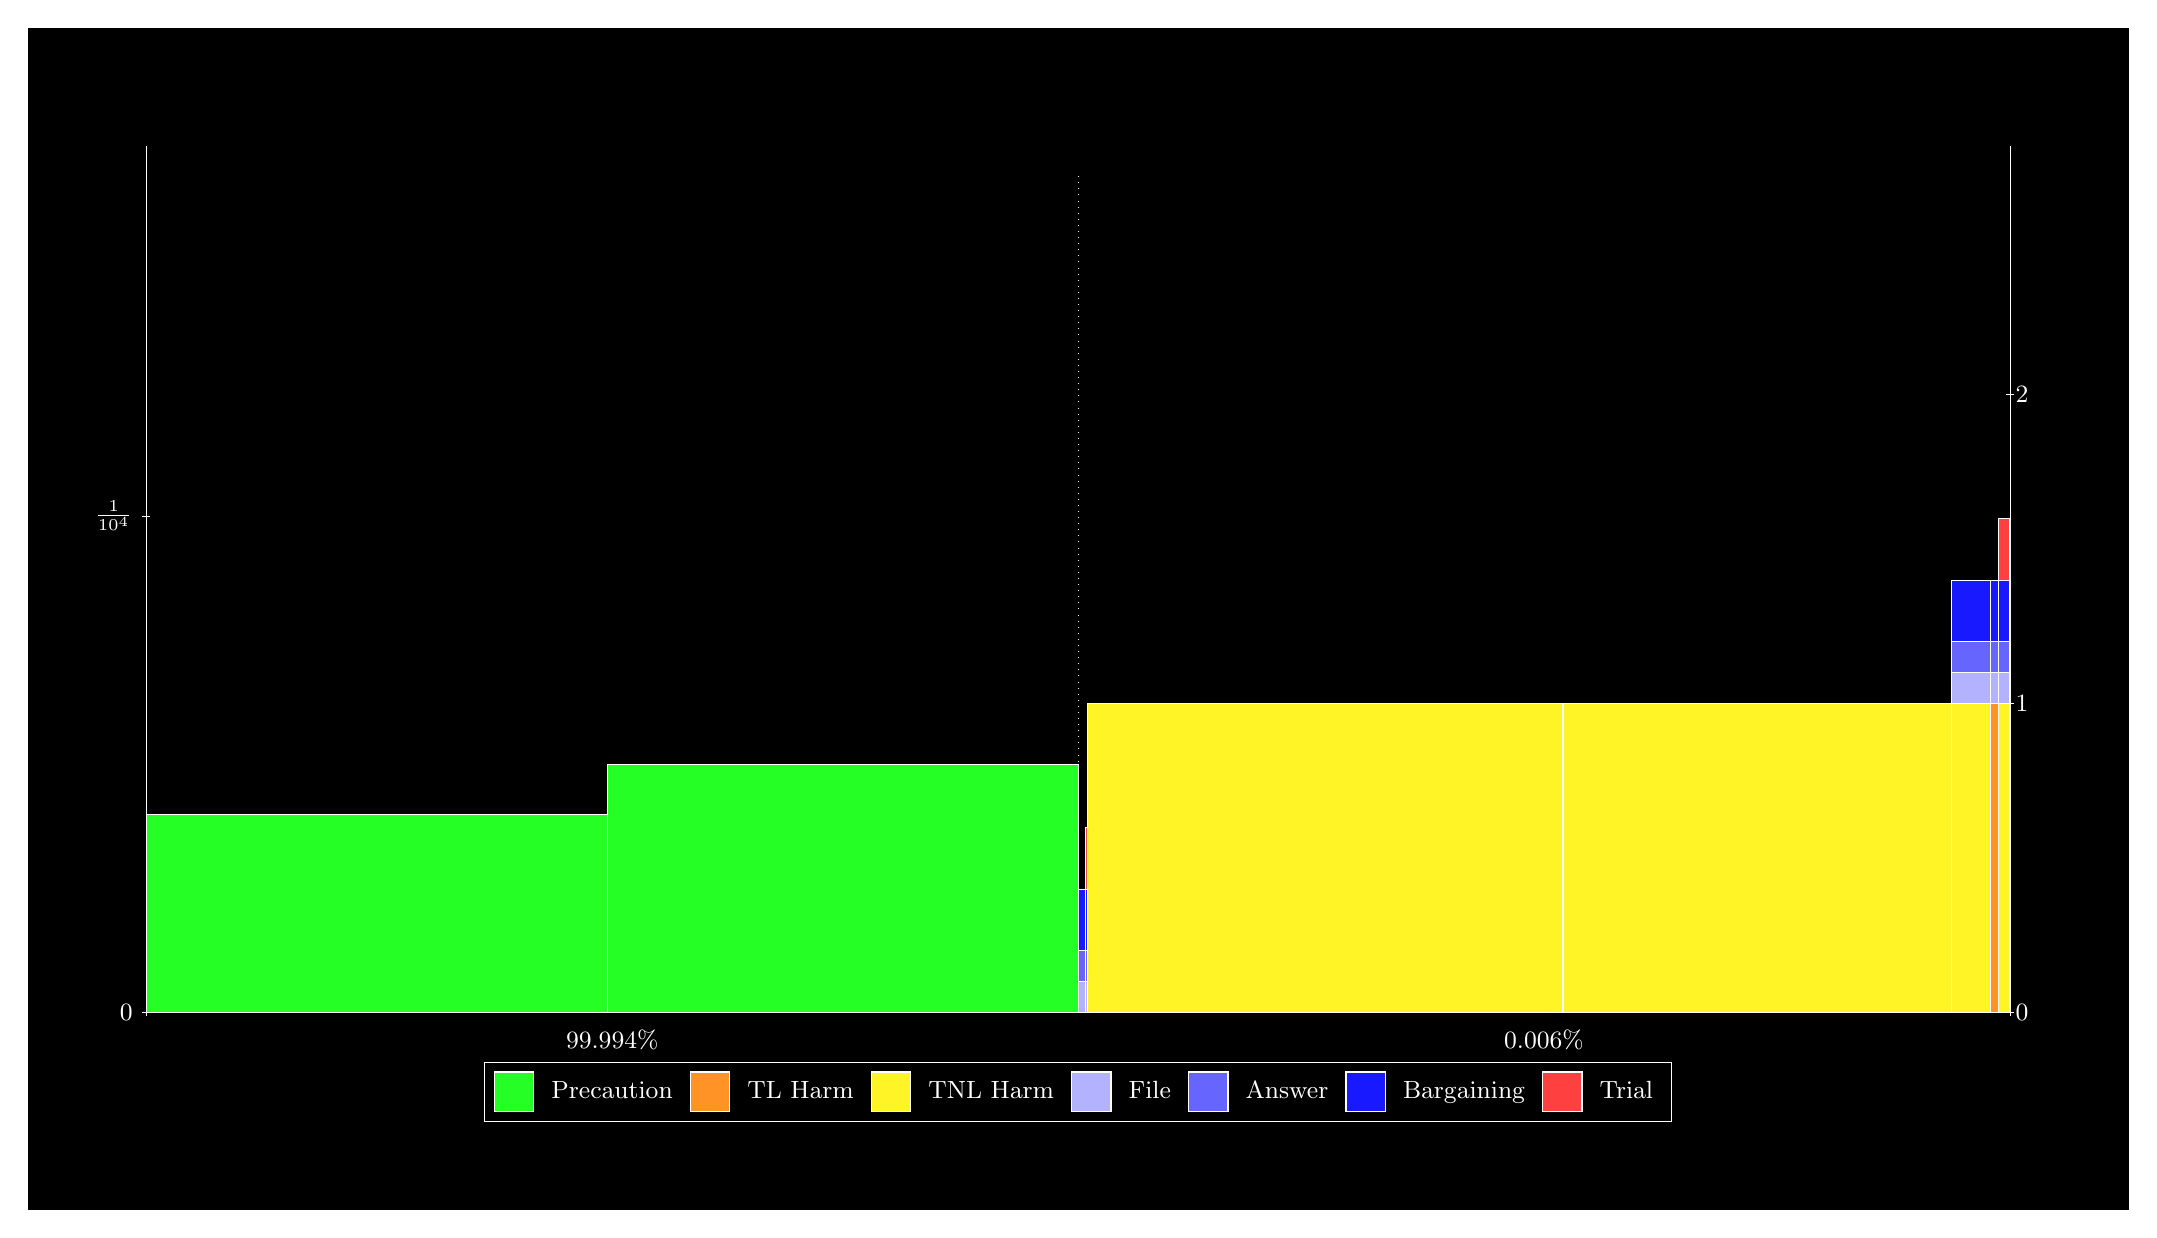
\begin{tikzpicture}
\draw[fill=black] (0,0) rectangle (26.667,15);
\draw[fill=green!85,draw=white,very thin] (1.5,2.5) rectangle (7.3571,5.0223);
\draw[fill=green!85,draw=white,very thin] (7.3571,2.5) rectangle (13.333,5.6529);
\draw[fill=green!85,draw=white,very thin] (13.333,2.5) rectangle (13.43,2.5002);
\draw[fill=blue!30,draw=white,very thin] (13.333,2.5002) rectangle (13.43,2.8926);
\draw[fill=blue!60,draw=white,very thin] (13.333,2.8926) rectangle (13.43,3.2851);
\draw[fill=blue!90,draw=white,very thin] (13.333,3.2851) rectangle (13.43,4.0701);
\draw[fill=green!85,draw=white,very thin] (13.43,2.5) rectangle (13.452,2.5002);
\draw[fill=blue!30,draw=white,very thin] (13.43,2.5002) rectangle (13.452,2.8926);
\draw[fill=blue!60,draw=white,very thin] (13.43,2.8926) rectangle (13.452,3.2851);
\draw[fill=blue!90,draw=white,very thin] (13.43,3.2851) rectangle (13.452,4.0701);
\draw[fill=red!75,draw=white,very thin] (13.43,4.0701) rectangle (13.452,4.855);
\draw[fill=green!85,draw=white,very thin] (13.452,2.5) rectangle (19.481,2.5002);
\draw[fill=yellow!85,draw=white,very thin] (13.452,2.5002) rectangle (19.481,6.425);
\draw[fill=green!85,draw=white,very thin] (19.481,2.5) rectangle (19.495,2.5002);
\draw[fill=orange!85,draw=white,very thin] (19.481,2.5002) rectangle (19.495,6.425);
\draw[fill=green!85,draw=white,very thin] (19.495,2.5) rectangle (24.422,2.5002);
\draw[fill=yellow!85,draw=white,very thin] (19.495,2.5002) rectangle (24.422,6.425);
\draw[fill=green!85,draw=white,very thin] (24.422,2.5) rectangle (24.921,2.5002);
\draw[fill=yellow!85,draw=white,very thin] (24.422,2.5002) rectangle (24.921,6.425);
\draw[fill=blue!30,draw=white,very thin] (24.422,6.425) rectangle (24.921,6.8174);
\draw[fill=blue!60,draw=white,very thin] (24.422,6.8174) rectangle (24.921,7.2099);
\draw[fill=blue!90,draw=white,very thin] (24.422,7.2099) rectangle (24.921,7.9949);
\draw[fill=green!85,draw=white,very thin] (24.921,2.5) rectangle (25.015,2.5002);
\draw[fill=orange!85,draw=white,very thin] (24.921,2.5002) rectangle (25.015,6.425);
\draw[fill=blue!30,draw=white,very thin] (24.921,6.425) rectangle (25.015,6.8174);
\draw[fill=blue!60,draw=white,very thin] (24.921,6.8174) rectangle (25.015,7.2099);
\draw[fill=blue!90,draw=white,very thin] (24.921,7.2099) rectangle (25.015,7.9949);
\draw[fill=green!85,draw=white,very thin] (25.015,2.5) rectangle (25.164,2.5002);
\draw[fill=yellow!85,draw=white,very thin] (25.015,2.5002) rectangle (25.164,6.425);
\draw[fill=blue!30,draw=white,very thin] (25.015,6.425) rectangle (25.164,6.8174);
\draw[fill=blue!60,draw=white,very thin] (25.015,6.8174) rectangle (25.164,7.2099);
\draw[fill=blue!90,draw=white,very thin] (25.015,7.2099) rectangle (25.164,7.9949);
\draw[fill=red!75,draw=white,very thin] (25.015,7.9949) rectangle (25.164,8.7798);
\draw[fill=green!85,draw=white,very thin] (25.164,2.5) rectangle (25.167,2.5002);
\draw[fill=orange!85,draw=white,very thin] (25.164,2.5002) rectangle (25.167,6.425);
\draw[fill=blue!30,draw=white,very thin] (25.164,6.425) rectangle (25.167,6.8174);
\draw[fill=blue!60,draw=white,very thin] (25.164,6.8174) rectangle (25.167,7.2099);
\draw[fill=blue!90,draw=white,very thin] (25.164,7.2099) rectangle (25.167,7.9949);
\draw[fill=red!75,draw=white,very thin] (25.164,7.9949) rectangle (25.167,8.7798);
\draw[white,very thin] (1.5,2.5) -- (1.5,13.5);
\draw[white,very thin] (1.45,2.5) -- (1.55,2.5);
\node[font=\small,text=white, anchor=east] at (1.45, 2.5) {0};
\draw[white,very thin] (1.45,8.8057) -- (1.55,8.8057);
\node[font=\small,text=white, anchor=east] at (1.45, 8.8057) {$\frac{1}{10^{4}}$};

\draw[white,dotted,very thin] (13.333,2.83) -- (13.333,13.17);
\draw[white,very thin] (25.167,2.5) -- (25.167,13.5);
\draw[white,very thin] (25.117,2.5) -- (25.217,2.5);
\node[font=\small,text=white, anchor=west] at (25.117, 2.5) {0};
\draw[white,very thin] (25.117,6.4248) -- (25.217,6.4248);
\node[font=\small,text=white, anchor=west] at (25.117, 6.4248) {1};
\draw[white,very thin] (25.117,10.35) -- (25.217,10.35);
\node[font=\small,text=white, anchor=west] at (25.117, 10.35) {2};

\draw[white,very thin] (1.5,2.5) -- (25.167,2.5);
\draw[white,very thin] (1.5,2.45) -- (1.5,2.55);
\node[font=\small,text=white, anchor=north] at (1.5, 2.45) {};
\draw[white,very thin] (25.167,2.45) -- (25.167,2.55);
\node[font=\small,text=white, anchor=north] at (25.167, 2.45) {};

\node[font=\small,text=white,anchor=south] at (7.4167, 1.9) {99.994\%};
\node[font=\small,text=white,anchor=south] at (19.25, 1.9) {0.006\%};
\draw (13.3333,2.5) node (B) {};
\begin{scope}[align=center]
\matrix[scale=0.5,draw=white,below=0.5cm of B,nodes={draw},column sep=0.1cm]{
\node[rectangle,draw,minimum width=0.5cm,minimum height=0.5cm,fill=green!85]{}; & \node[draw=none,font=\small,text=white]{Precaution}; &
\node[rectangle,draw,minimum width=0.5cm,minimum height=0.5cm,fill=orange!85]{}; & \node[draw=none,font=\small,text=white]{TL Harm}; &
\node[rectangle,draw,minimum width=0.5cm,minimum height=0.5cm,fill=yellow!85]{}; & \node[draw=none,font=\small,text=white]{TNL Harm}; &
\node[rectangle,draw,minimum width=0.5cm,minimum height=0.5cm,fill=blue!30]{}; & \node[draw=none,font=\small,text=white]{File}; &
\node[rectangle,draw,minimum width=0.5cm,minimum height=0.5cm,fill=blue!60]{}; & \node[draw=none,font=\small,text=white]{Answer}; &
\node[rectangle,draw,minimum width=0.5cm,minimum height=0.5cm,fill=blue!90]{}; & \node[draw=none,font=\small,text=white]{Bargaining}; &
\node[rectangle,draw,minimum width=0.5cm,minimum height=0.5cm,fill=red!75]{}; & \node[draw=none,font=\small,text=white]{Trial}; \\\\
};\end{scope}

\end{tikzpicture}
\end{document}